\chapter{Application to ARMA processes}

The application of TDA to time series analysis is well established (\cite{perea_sliding_2015})\todo{cite papers about TDA for time series}. A prominent example that shows the connection between these two fields clearly are (noisy) sine curves: at the right scale, the two dimensional sliding window reveals a loop. See \cite{KARAN2021115326}

In the first section, we give an overview on the theory of time series needed for our purposes. Next we discuss the embedding of time series as point clouds in $\mathbb{R}^k$, where Takens' theorem will play an important role. Finally, we present our numerical results and interpret them.

\todo[inline]{Main Question: Sequence of what?}

\todo[inline]{TDA and Sliding window embedding not even needed?}

\todo[inline]{Main goal: Prove consistency of spectrally selected order $k^{\star}$ to the true order $p$}

\section{Preliminaries on time series}

For information on autoregressive moving-average (ARMA) models, see Brockwell et al~\cite[Chapter~3]{brockwell2016introduction}. 

We consider a family of random variables $(Z_t)_{t\in\mathbb{Z}}$ that has the following properties:
\begin{subequations}\label{eq:white-noise-assumptions}
    \begin{align}
        \mathbb{E}[Z_t] &= 0,
        && t\in\mathbb{Z}, \label{eq:white-noise-centered}\\
        \operatorname{Var}[Z_t] &= \sigma^2\in(0,+\infty),
        && t\in\mathbb{Z}, \label{eq:white-noise-variance}\\
        \operatorname{Cov}[Z_t,Z_s] &= 0,
        && t,s\in\mathbb{Z},\ t\neq s. \label{eq:white-noise-uncorrelated}
    \end{align}
\end{subequations}

Later, we will drop the finite variance assumption~\eqref{eq:white-noise-variance} and replace the uncorrelated assumption~\eqref{eq:white-noise-uncorrelated} with independence.

For the innovations $Z_t$, we will consider the following distributions:
\begin{itemize}
    \item Uniform: $Z_t\sim\mathcal{U}[-a,a]$ for some $a>0$ (variance: $\operatorname{Var}[Z_t]=a^2/3$)
    \item Normal: $Z_t\sim\mathcal{N}(0,\sigma^2)$
    \item Student-t: $Z_t\sim t_{\nu}$ for some degrees of freedom $\nu>0$ (the variance does not exist for $\nu\le2$)
\end{itemize}

The last distribution is part of a more general kind of distributions that fulfills
\begin{align*}
    \mathbb{P}(|Z|>x)=x^{-\alpha}L(x)
\end{align*}
for some $\alpha\in(0,2)$ and a slowly varying function $L$. 

\todo[inline]{establish hierarchy: alpha stable, slowly varying property, heavy tails}

Some common heavy tailed distributions are
\begin{itemize}
    \item Cauchy: $X\sim C(x_0,\gamma)$
    \item Levy: $X\sim L()$
    \item Pareto: $X\sim P()$
    \item Student-t: $X\sim t_{\nu}$
\end{itemize}

\begin{Def}
    Let $(Z_t)_{t\in\mathbb{Z}}$ be a family of random variables satisfying the assumptions~\eqref{eq:white-noise-assumptions}. A process $(X_t)$ is an ARMA($p$, $q$) process if
    \begin{align}\label{eq:def_arma}
        X_t=\sum_{i=1}^{p}\phi_iX_{t-i}+Z_t+\sum_{j=1}^{q}\theta_jZ_{t-j}, && t\in\mathbb{Z},
    \end{align}
    where the polynomials $\phi(z):=1-\phi_1z-\dots-\phi_pz^{p}$ and $\theta(z):=1+\theta_1z+\dots+\theta_qz^{q}$ are required to have no common factors. Additionally, $\phi_p\neq0$ and $\theta_q\neq0$.
\end{Def}

In case of $\theta\equiv1$ we recover the autoregressive (AR) process of order $p\in\mathbb{N}$ and $X_t$ has the form
\begin{align}\label{eq:ar(p)}
    X_t=\sum_{i=1}^{p}\phi_iX_{t-i}+Z_t,
\end{align}
where $\phi_i\in\mathbb{R}$ are the coefficients with $\phi_p\ne0$.

It is well known that there exists a stationary process $(X_t)_{t\in\mathbb{Z}}$ that can be written in the form \eqref{eq:def_arma} if $\phi(z)\neq0$ for all $z\in\mathbb{C},\lvert z\rvert=1$. Another important property that we will need for the geometric interpretation of the embedded AR process is causality: An ARMA process $(X_t)$ is called causal if there exist constants $\psi_j$ with $\sum_j|\psi_j|<+\infty$, such that $X_t=\sum_{j=0}^{\infty}\psi_jZ_{t-j}$ for all $t\in\mathbb{Z}$. It turns out that this property is stronger than stationarity, as an ARMA process is causal iff $\phi(z)\neq0$ for all $z\in\mathbb{C},\lvert z\rvert\le1$. In what follows, we will exclusively work with causal ARMA processes.

For our experiments, we use random coefficients $\theta_1,\dots,\theta_q\sim\mathcal{U}[-1,1]$ since there are no restrictions on these coefficients for the ARMA process to be causal. For the AR coefficients, we will first draw $\phi'_1,\dots,\phi'_p\sim\mathcal{U}[-1,1]$ and then set $\phi_i=\text{sc}\cdot\phi_i'/\|\phi'\|_1$ for some scale parameter $\text{sc}<1$. This is a necessary condition for the generated AR($p$) processes to be causal.

\todo[inline]{Find sufficient condition implementation}

\todo[inline]{Discuss automatic coefficient selection}

\section{Order selection methods}

There are several established methods for choosing an order $\hat{p}$ given a realization $X=(X_1,\dots,X_T)$ that is assumed to come from an AR($p$) process. 

\begin{itemize}
    \item Final Prediction Error (FPE) Criterion
    \item Akaike Information Criterion (AIC)
    \item Bayesian Information Criterion (BIC)
\end{itemize}

\todo[inline]{Are there any guarantees for the quality of such selectors?}

\todo[inline]{order selection for heavy tailed innovations? Look for papers}

Once the order has been chosen, the AR coefficients $\phi_1,\dots,\phi_{\hat{p}}$ can be estimated using one of the following classical procedures:
\begin{itemize}
    \item Yule-Walker Estimation
    \item Burg's Algorithm
    \item The Hannan-Rissanen Algorithm
    \item Maximum Likelihood Estimation
\end{itemize}



\section{Embedding of time series}

In order to apply machinery from Topological Data Analysis to time series data, one has to embed the time series into $\mathbb{R}^k$ for some embedding dimension $k\in\mathbb{N}$. The main method for this is the so called sliding-window embedding (see~\cite{perea_sliding_2015}), which we will describe in detail now. Let $X=(X_1,\dots,X_T)$ be one realization of some univariate time series. Then we obtain a point cloud from $X$ by defining:
\begin{align*}
    Y_t^{(k)}&=\begin{pmatrix}
        X_{t}\\
        X_{t+1}\\
        \vdots\\
        X_{t+k-1}
    \end{pmatrix}\in\mathbb{R}^k\\ 
    \mathcal{P}_{k}&=\left\{Y_t^{(k)}:t=1,\dots,T-k_{\max}+1\right\}\subseteq\mathbb{R}^k
\end{align*}
Here, $k\in\mathbb{N}$ is the dimensionality of the point cloud $\mathcal{P}_{k}$ and $k_{\max}$ a predetermined upper cap, that is, $k\in\{1,\dots,k_{\max}\}$.

\todo[inline]{Give discussion why it does not matter if we consider the past or future $k$ observations for the geometry of the point cloud (forward versus backward embedding)}

Takens' Theorem mainly serves as a theoretical justification or motivation for the sliding-window embedding.

\begin{Thm}[Takens]
    Let $\mathcal{M}$ be a compact manifold of dimension $m$. Let $\phi\in\operatorname{Diff}^2(\mathcal{M})$ and $y\in C^2(\mathcal{M},\mathbb{R})$. Then the map $\Phi_{(\phi,y)}:\mathcal{M}\to\mathbb{R}^{2m+1}$ defined by
    \begin{align*}
        \Phi_{(\phi,y)}(x)=\begin{pmatrix}
            y(x)\\
            y(\phi(x))\\
            \vdots\\
            y(\phi^{2m}(x))
        \end{pmatrix}
    \end{align*}
    is an embedding, given that the pair $(\phi,y)$ is generic.
\end{Thm}

\todo[inline]{connect Takens' Theorem better, add interpretation}

\todo[inline]{study time dynamics, formation of loops, $t$ vs number of loops until $t$, size of loops (how many time steps before loop closes)}

\section{Scale Selection for the AR-process application}

Consider the sequence of point clouds $\mathcal{P}_k$ with increasing dimension $k\in\mathbb{N}$. Our goal is to apply the scale selection principle presented in Chapter~\ref{chap:methodology} to determine an \enquote{optimal} scale $k^{\star}\in\{1,\dots,k_{\max}\}$. In order to apply the scale selection, we need to construct a sequence (not necessarily a filtration) of simplicial complexes $\{L_k\}_{k=1}^{k_{\max}}$. Afterwards, we need to choose what kind of operation $\oplus$ we use to combine the simplicial complexes and the right type of functional (preferably of topological nature) to evaluate the simplicial complexes. In the end, we want to find a triple $(f,\{K_k\}_{k=1}^{k_{\max}},\oplus)$ that is spectrally optimizable.

\enquote{Optimality} of $k^{\star}$ should encompass $k^{\star}=p$ or at least $k^{\star}\approx p$ where the meaning of $\approx$ is specified. In particular, this \enquote{optimal} scale selection serves as an order estimation method without requiring the existence of (second) moments of the innovations.

\subsection*{Dimension lift}

The first step is to lift the point clouds $\mathcal{P}_k$, $k=1,\dots,k_{\max}$ to a common ambient dimension. That is, transforming each $\mathcal{P}_k$ to $\mathcal{Q}_k\subseteq\mathcal{R}^{k_{\max}}$. In order to do this, we split the observed time series $X=(X_1,\dots,X_T)$ into a train and test part:
\begin{align*}
    X_{\text{train}}&=(X_1,\dots,X_{T'})\\
    X_{\text{test}}&=(X_{T'+1},\dots,X_T)
\end{align*}

For $k\in\{1,\dots,k_{\max}\}$ we complete $Y_{t}^{(k)}=(X_t,X_{t+1},\dots,X_{t+k-1})^{T}\in\mathbb{R}^{k}$ to
\begin{align*}
    p_{t}^{(k)}&=\begin{pmatrix}
        I_k\\
        \hat{A}_k
    \end{pmatrix}Y_t^{(k)}=\begin{pmatrix}
        Y_{t}^{(k)}\\
        \hat{A}_kY_{t}^{(k)}
    \end{pmatrix}\\
    &=\begin{pmatrix}
        X_t\\
        X_{t+1}\\
        \vdots\\
        X_{t+k-1}\\
        \hat{\alpha}_{1,1}^{(k)}X_t+\dots+\hat{\alpha}_{1,k}^{(k)}X_{t+k-1}\\
        \vdots\\
        \hat{\alpha}_{k_{\max}-k,1}^{(k)}X_{t}+\dots+\hat{\alpha}_{k_{\max}-k,k}^{(k)}X_{t+k-1}
    \end{pmatrix}\in\mathbb{R}^{k_{\max}},\\
    t&=T'+1,\dots,T-k_{\max}+1,
\end{align*}
where $I_k\in\mathbb{R}^{k\times k}$ is the identity matrix and $\hat{A}_k\in\mathbb{R}^{(k_{\max}-k)\times k}$ a linear completion matrix with coefficients $\hat{\alpha}_{i,j}^{(k)}$, $i=1,\dots,k_{\max}-k$, $j=1,\dots,k$. The completed part $\hat{A}_kY_{t}^{(k)}$ resembles $z_t^{(k)}=(X_{t+k},\dots,X_{t+k_{\max}-1})^{T}\in\mathbb{R}^{k_{\max}-k}$ (the next $k_{\max}-k$ observations after $Y_t^{(k)}$).

We determine $\hat{A}_k$ by minimizing a functional $\Psi_k(A_k)$ that depends on the train data $X_{\text{train}}$. The kind of functional depends on the nature of the innovation distribution. For example, we might choose different $\Psi_k$ depending on whether the innovations are light tailed or heavy tailed. Afterwards, we set $\hat{z}_t^{k}=\hat{A}_kY_{t}^{(k)}$ and $p_t^{k}=(Y_{t}^{(k)},\hat{z}_t^{k})$. We denote the lifted point cloud by $\mathcal{Q}_k=\{p_t^{k}:t=k_{\max},\dots,T\}$.


We are interested in the geometry of the point cloud $\mathcal{Q}_k$. We write
\begin{align*}
    p_t^{(k)}&=\sum_{j=1}^{k}X_{t-j+1}\cdot h_j, & h_j=\begin{pmatrix}
        e_j\\
        \hat{\alpha}_{1,j}\\
        \vdots\\
        \hat{\alpha}_{k_{\max}-k,j}
    \end{pmatrix},
\end{align*}
where $e_j$ is the $j$-th unit vector in $\mathbb{R}^{k}$. Note that the directions $h_1,\dots,h_k$ are independent of $t$. Therefore, $\mathcal{Q}_k$ is contained in a $k$-dimensional linear subspace of $\mathbb{R}^{k_{\max}}$, namely $\operatorname{span}\{h_1,\dots,h_k\}$.

Note that we have the following equation:
\begin{align}\label{eq:squared_2norm_of_lifted_points}
    \left(p_t^{(k)}-p_s^{(k)}\right)^{T}\left(p_t^{(k)}-p_s^{(k)}\right)&=\left(Y_t^{(k)}-Y_s^{(k)}\right)^{T}\left(I_k+\hat{A}_k^{T}\hat{A}_k\right)\left(Y_t^{(k)}-Y_s^{(k)}\right).
\end{align}
% Linear completion changes metric according to how strongly observed coordinates predict missing coordinates

We have
\begin{align*}
    M_t^{(k)}\cdot\begin{pmatrix}
        X_T\\
        \vdots\\
        X_1
    \end{pmatrix}=
    p_t^{(k)},
\end{align*}
where the matrix $M_t^{(k)}\in\mathbb{R}^{k_{\max}\times T}$ is given by
\begin{align*}
    \begin{pmatrix}
        \mathbf{0} & I_k & \mathbf{0}\\
        \mathbf{0} & \hat{A}_k & \mathbf{0}
    \end{pmatrix},
\end{align*}
with $\mathbf{0}$ being matrices of the right size that contain only zeros.

\subsubsection*{Dimension lift via Least Squares (Light tailed case)}

In case of light tailed innovations, we can determine the linear completion matrix by Ordinary Least Squares (see the book~\cite{Grey_1981} for information on OLS with a vector valued response). That is, we determine
\begin{align}\label{eq:ls_dimension_lift}
    \hat{A}_k\in\arg\min\left\{\sum_{t=1}^{T'-k_{\max}+1}\left\|z_t^{(k)}-AY_{t}^{(k)}\right\|_2^2:A\in\mathbb{R}^{(k_{\max}-k)\times k}\right\}.
\end{align}
The Problem~\eqref{eq:ls_dimension_lift} can be formulated in a more compact way using matrix notation. To this end, we introduce the matrices
\begin{align*}
    Y_k&=\begin{pmatrix}
        Y_{1}^{(k)} & \cdots & Y_{T'-k_{\max}+1}^{(k)}
    \end{pmatrix}\in\mathbb{R}^{k\times(T'-k_{\max}+1)}\\
    Z_k&=\begin{pmatrix}
        z_{1}^{(k)} & \cdots & z_{T'-k_{\max}+1}^{(k)}
    \end{pmatrix}\in\mathbb{R}^{(k_{\max}-k)\times(T'-k_{\max}+1)}
\end{align*}
and Problem~\eqref{eq:ls_dimension_lift} becomes
\begin{align*}
    \hat{A}_k\in\arg\min\left\{\operatorname{tr}\left((Z_k-AY_k)^{T}(Z_k-AY_k)\right):A\in\mathbb{R}^{(k_{\max}-k)\times k}\right\}.
\end{align*}



The solution can be written down explicitly:
\begin{align*}
    \hat{A}_k&=Z_kY_k^{T}\left(Y_kY_k^{T}\right)^{-1}\\&
    =\underbrace{\sum_{t=1}^{T'-k_{\max}+1}z_t^{(k)}\left(Y_t^{(k)}\right)^T}_{=U_k}\left(\underbrace{\sum_{t=1}^{T'-k_{\max}+1}Y_t^{(k)}\left(Y_t^{(k)}\right)^{T}}_{=V_k}\right)^{-1},
\end{align*}
provided that $V_k=Y_kY_k^{T}$ is invertible. This is almost surely the case if the innovations have an absolute continuous distribution.

\todo[inline]{Prove $\mathbb{P}(Y_kY_k^{T}\text{ is invertible})=1$ explicitly}

% cite Mityagin

The entries of the matrices $U_k=(U_{ij}^{(k)})\in\mathbb{R}^{(k_{\max}-k)\times k}$ and $V_k=(V_{ij}^{(k)})\in\mathbb{R}^{k\times k}$ can be written as
\begin{align*}
    U_{ij}^{(k)}&=\sum_{t=1}^{T'-k_{\max}+1}X_{t+k+i-1}X_{t+j-1},\quad i=1,\dots,k_{\max}-k,j=1,\dots,k\\
    V_{ij}^{(k)}&=\sum_{t=1}^{T'-k_{\max}+1}X_{t+i-1}X_{t+j-1},\quad i,j=1,\dots,k
\end{align*}
By the ergodic theorem (??) these entries converge and their limit is determined by the auto-covariance function $\gamma$ of the process $(X_t)$:
\begin{align*}
    \tilde{U}_{ij}^{(k)}&=\frac{1}{T-k_{\max}+1}U_{ij}^{(k)}\stackrel{T\to\infty}{\to}\mathbb{E}\left[X_{t+k+i-1}X_{t+j-1}\right]=\gamma(j-i-k)\\
    \tilde{V}_{ij}^{(k)}&=\frac{1}{T-k_{\max}+1}V_{ij}^{(k)}\stackrel{T\to\infty}{\to}\mathbb{E}\left[X_{t+i-1}X_{t+j-1}\right]=\gamma(j-i)
\end{align*}
Thus we have the following convergence, which is understood component wise:
\begin{align*}
    \hat{A}_k=U_kV_k^{-1}\stackrel{T\to\infty}{\to}\operatorname{Cov}\left[z_t^{(k)},Y_t^{(k)}\right]\left(\operatorname{Cov}\left[Y_t^{(k)}\right]\right)^{-1}.
\end{align*}


The uncompleted part $z_t^{(k)}$ can be expressed as a linear function of $Y_t^{(k)}$ and innovations $Z=(Z_{t+k},\dots,Z_{t+k_{\max}-1})$ \textcolor{red}{once $k\ge p$}. That is, there exist matrices $B_k$ and $C_k$ such that $z_t^{(k)}=B_kY_t^{(k)}+C_kZ$. This is not surprising because linearity is already part of the AR process. Thus, our linear prediction $\hat{z}_t^{(k)}=\hat{A}_kY_t^{(k)}$ is a natural choice.

The matrices $B_k$ and $C_k$ can be determined by first writing
\begin{align*}
    &H_k\begin{pmatrix}
        Y_{t}^{(k)}\\
        z_t^{(k)}
    \end{pmatrix}=\begin{pmatrix}
        Z_{t+k}\\
        \vdots\\
        Z_{t+k_{\max}-1}
    \end{pmatrix}\\&
    z_t^{(k)}=-H_z^{-1}H_YY_t^{(k)}-H_z^{-1}\begin{pmatrix}
        Z_{t+k}\\
        \vdots\\
        Z_{t+k_{\max}-1}
    \end{pmatrix}
\end{align*}
with
\begin{align*}
    H_k=\begin{pmatrix}
        0 & \cdots & 0 & \phi_p & \phi_{p-1} & \cdots & \phi_1 & 1 & 0 & \cdots & 0\\
        0 & \cdots & 0 & 0 & \phi_p & \phi_{p-1} & \cdots & \phi_1 & 1 & \cdots & 0\\
        \vdots & & \vdots & \vdots & \ddots & \ddots & \ddots & & \ddots & \ddots & \vdots\\
        0 & \cdots & 0 & 0 & \cdots & 0 & \phi_p & \phi_{p-1} & \cdots & \phi_1 & 1
    \end{pmatrix}
\end{align*}
and reconstruction matrix $B_k=-H_z^{-1}H_Y$, where $H_p^{(k)}=(H_Y H_z)$. Note that $H_z$ is in fact invertible since it is a lower triangular matrix with all diagonal elements being equal to $1$.

\todo[inline]{What about a representation in the case $k<p$}

\subsubsection*{Dimension lift via Excursion metric minimization}

\begin{itemize}
    \item $F_0\sim X_t$? Take empirical cdf
    \item When is $X_t$ ergodic?
\end{itemize}

We again have an observed time series $X=(X_{1},\dots,X_T)$ that is split up into $X_{\text{train}}=(X_1,\dots,X_{T_{\text{train}}})$ and $X_{\text{test}}=(X_{T_{\text{train}}+1},\dots,X_T)$. Define $X^{\text{test}}_t=X_{T_{\text{train}}+t}$ for $t=1,\dots,T-T_{\text{train}}$. The goal is to lift $Y_t^{(k)}$ for $t=T_{\text{train}}+1,\dots,T$ from $\mathbb{R}^k$ to $\mathbb{R}^{k_{\max}}$. Denote the lifted point by $p_t^{(k)}$. It is given by
\begin{align*}
    p_t^{(k)}=\begin{pmatrix}
        X_{t}\\
        X_{t+1}\\
        \vdots\\
        X_{t+k-1}\\
        \hat{X}_{t+k}\\
        \vdots\\
        \hat{X}_{t+k_{\max}-1}
    \end{pmatrix}
\end{align*}
with
\begin{align*}
    \hat{X}_{t+k-1+m}=\sum_{j=1}^{k}\lambda_j^{(m)}X_{t+j-1}, && m=1,\dots,k_{\max}-k
\end{align*}
The coeficients $\lambda_j^{(m)}$ are determined by
\begin{align*}
    \hat{\lambda}^{(m)}&\in\arg\min\left\{\mathcal{E}(X_{t+k-1+m},\hat{X}_{t+k-1+m})\right\}
\end{align*}
We have
\begin{align*}
    \mathcal{E}(X_{t+k-1+m},\hat{X}_{t+k-1+m})&=2\mathbb{E}\left[F(X_{t+k-1+m})\vee F(\hat{X}_{t+k-1+m})\right]\\&
    -\mathbb{E}\left[F(\hat{X}_{t+k-1+m})\right]-\frac{1}{2}
\end{align*}

The empirical version is
\begin{align*}
    \Phi(\lambda)&=\frac{2}{T_{\text{train}}-k_{\max}+1}\sum_{s=1}^{T_{\text{train}}-k_{\max}+1}F_{\hat{\theta}}\left(\sum_{j=1}^{k}\lambda_jX_{s-1+j}\right)\vee F_{\hat{\theta}}\left(X_{s+k-1+m}\right)\\&
    -\frac{2}{T_{\text{train}}-k_{\max}+1}\sum_{s=1}^{T_{\text{train}}-k_{\max}+1}F_{\hat{\theta}}\left(\sum_{j=1}^{k}\lambda_jX_{s-1+j}\right)-\frac{1}{2}
\end{align*}
where $F_{\hat{\theta}}$ is the empirical cumulative distribution function fitted on the data $X_{\text{train}}$.

\subsection*{Simplicial complex construction}

\begin{itemize}
    \item Temporal geometric complexes: $D_k(s,t)=\|Y_s^{(k)}-Y_t^{(k)}\|\le\epsilon_k$
    \item $E_k=\{\{s,t\}:D_k(s,t)\le\epsilon_k\}$, $\Sigma_{kl}=|E_k\cap E_l|$, $\Sigma_{kl}=|E_k\cap E_l|/|E_k\cup E_l|$
    \item $K_k=\operatorname{Flag}(V,E_k)$, $\Sigma_{kl}=f(K_k)+f(K_l)-f(K_k\cup K_l)$
    \item build $K_k$ from prediction errors, excursion distances or dependence scores
    \item $\oplus=\triangle$ (symmetric difference)
    \item $w_k(s,t)=d(\mathcal{L}(X_{s+k}|Y_s^{(k)}),\mathcal{L}(X_{t+k}|Y_t^{(k)}))$
\end{itemize}

\todo[inline]{give precedence: ordered temporal simplex, simplex generated by a directed path through time}

\todo[inline]{Does the clique closure performed by the flag complex preserve the information we care about? Many different weighted graphs can have exactly the same flag complex. We may actually lose information.}

A general construction principle can be described in a graph theoretical way. Consider the set of vertices $V=\{T_{\text{train}}+1,\dots,T-k_{\max}+1\}$. Two distinct time indices $s$ and $t$ form an edge if $w_k(s,t)\le\tau$, where $w_k:V\times V\to\mathbb{R}_{\ge0}$ is a weight function and $\tau>0$ some threshold parameter. Information about linear dependence enters via the choice of the weight function $w_k$. Let $E_k^{\tau}$ be the set of edges and $G_k^{\tau}=(V,E_k^{\tau})$ the resulting graph.

Now we take the flag complex $L_k^{\tau}=\text{Flag}(G_k^{\tau})$ and obtain a sequence of complexes $\{L_k^{\tau}\}_{k=1}^{k_{\max}}$. In order for $\{L_k\}_{k=1}^{k_{\max}}$ to be a filtration, it must hold
\begin{align*}
    w_{k+1}(e)\le w_{k}(e),&&\forall e\in E_k\text{ and }k=1,\dots,k_{\max}-1.
\end{align*}
At the moment, it is not clear whether the specific weighting choices discussed below fulfill this property.

The first candidate for $w_k$ is a norm of the covariance matrix. To this end, compute the covariance matrix:
\begin{align*}
    D_{s,t}^{(k)}=\operatorname{Cov}\left[p_t^{(k)},p_s^{(k)}\right]&=\begin{pmatrix}
        I_k\\
        \hat{A}_k
    \end{pmatrix}C_{s,t}^{(k)}\begin{pmatrix}
        I_k & \hat{A}_k^{T}
    \end{pmatrix}
\end{align*}

\begin{align*}
    C_{s,t}^{(k)}&=\operatorname{Cov}\left[Y_s^{(k)},Y_t^{(k)}\right]\\&=
    \begin{pmatrix}
        \mathbb{E}[X_sX_t] & \mathbb{E}[X_sX_{t+1}] & \cdots & \mathbb{E}[X_sX_{t+k-1}]\\
        \vdots & \vdots & & \vdots\\
        \mathbb{E}[X_{s+k-1}X_t] & \mathbb{E}[X_{s+k-1}X_{t+1}] & \cdots & \mathbb{E}[X_{s+k-1}X_{t+k-1}]
    \end{pmatrix}\\&
    =\begin{pmatrix}
        \gamma(s-t) & \gamma(s-t-1) & \cdots & \gamma(s-t-k+1)\\
        \gamma(s-t+1) & \gamma(s-t) & \cdots & \gamma(s-t-k+2)\\
        \vdots & \vdots & \ddots & \vdots\\
        \gamma(s-t+k-1) & \gamma(s-t+k-2) & \cdots & \gamma(s-t)
    \end{pmatrix}
\end{align*}

We need a scalar summary:
\begin{align*}
    &\rho_k(s,t)=\|C_{s,t}^{(k)}\|_F^2\\
    &\eta_k(s,t)=\|D_{s,t}^{(k)}\|_F^2=\left(k+\|\hat{A}_k\|_F^2\right)^2\|C_{s,t}^{(k)}\|_F^2
\end{align*}

\todo[inline]{autocovariance $\gamma(h)$ can be expressed via $\phi_1,\dots,\phi_p$ by using the Yule-Walker-Equations}

In cases where the second moment does not exist, the covariance is no longer viable. In such cases, we may use
\begin{align*}
    w_k(s,t)=\|p_s^{(k)}-p_t^{(k)}\|_1.
\end{align*}



\subsection*{Assembly of the scale similarity matrix}

We try out two different constructions:
\begin{align*}
    \langle L_i, L_j\rangle_f=f(L_i)+f(L_j)-f(L_i\cup L_j),
\end{align*}
where $f$ must be sub-additive, since $\{L_k\}_{k=1}^{k_{\max}}$ is not a filtration in general, and
\begin{align*}
    \langle L_i,L_j \rangle_f=f(L_i\cup L_j),
\end{align*}
where $f$ is non-negative. The scale similarity matrix becomes
\begin{align*}
    \Sigma_{k_{\max}}=\begin{pmatrix}
        \langle L_1, L_1\rangle_f & \langle L_1, L_2\rangle_f & \dots & \langle L_1, L_{k_{\max}}\rangle_f\\
        \langle L_1, L_2\rangle_f & \langle L_2, L_2\rangle_f & \cdots & \langle L_2, L_{k_{\max}}\rangle_f\\
        \vdots & \vdots & \ddots & \vdots\\
        \langle L_1, L_{k_{\max}}\rangle_f & \langle L_2, L_{k_{\max}}\rangle_f & \dots & \langle L_{k_{\max}}, L_{k_{\max}}\rangle_f
    \end{pmatrix}.
\end{align*}
Let $v^*=(v^*_1,\dots,v^*_{k_{\max}})$ be the principal eigenvector of $\Sigma_{k_{\max}}$. The \enquote{optimal} scale is set to $k^{*}\in\arg\max\{v^*_k:k=1,\dots,k_{\max}\}$.

\subsection*{Choice of the Functional $f$}

As a simple starting point, we try functionals of the form
\begin{align*}
    f(K)=\delta|C(K)|^{\alpha}|E(K)|^{\xi}
\end{align*}
or alternatively any transformation of $f$ that preserves monotonicity:
\begin{align*}
    \tilde{f}(K)&=\log{f(K)}=\tilde{\delta}+\alpha\log{\left(|C(K)|\right)}+\xi\log{\left(|E(K)|\right)}
\end{align*}

\todo[inline]{Some functional that measures the volume of the complex in some sense and detects the flatness}

\todo[inline]{graph functionals, mutual information from graph functionals}

\section{Statistical Approach}

\todo[inline]{Keep working on this idea!}

We obtain estimates of the coefficients and consider the error
\begin{align*}
    \hat{\sigma}_k^2=\frac{1}{n}\sum_{t}\left(X_t-\sum_{j=1}^{k}\hat{\alpha}_j^{(k)}X_{t-j}\right)
\end{align*}

Define the function $f$ on the class $\mathcal{A}_k(\mathcal{D})$ of all AR processes of order $k$ with innovations coming from the distribution $\mathcal{D}$ by
\begin{align*}
    f(\mathcal{A}_k(\mathcal{D}))=\frac{n}{2}\hat{\sigma}_k^{2}+\lambda k
\end{align*}



\section{Numerical Experiments}



Multiple questions arise:
\begin{itemize}
    \item How does increasing $k_{\max}$ influence the selection of $k^*$
    \item For fixed $k_{\max}$, $\alpha$, $\xi$ can $\tau$ be found such that the correct scale is chosen
    \item For fixed $\tau$ and $k_{\max}$ can $\alpha$ and $\xi$ be tuned?
\end{itemize}

\newpage

\section{Geometric Approach}

\todo[inline]{Explain why this idea is \enquote{dead}. Move to possible appendix because it is sill a nice connection between time series analysis and convex geometry?}

In this section, we study how the geometry of the point cloud $\mathcal{P}_k\subseteq\mathbb{R}^{k}$ changes with increasing embedding dimension $k$. For simple innovation distributions, like uniform or normal, the point cloud $\mathcal{P}_k$ is characterized by well known convex--geometric objects. The question becomes if we can apply some convex--geometric functional $f$ to these well known objects and detect a transition at $k=p+1$, where $p$ is the AR order of the embedded time series.

In order to be able to talk about the \enquote{geometry of a point cloud} in a rigorous way, we first need to introduce some concepts from probability theory. Let $Y$ be a $d$-dimensional random vector with density $f_Y$. The \textit{support} of $Y$ is given by
\begin{align*}
    \operatorname{supp}(Y)=\{x\in\mathbb{R}^k:\mathbb{P}(Y\in B_r(x))>0\text{ for all }r>0\}
\end{align*}
In the case where $f_Y$ is continuous, it holds $\operatorname{supp}(Y)=\operatorname{cl}\{y\in\mathbb{R}^{k}:f_Y(y)>0\}$. The \textit{minimum volume set} (compare~\cite{JMLR:v7:scott06a}) is defined by
\begin{align*}
    E_{\alpha}\in\arg\min\{\lambda_d(A):\mathbb{P}(Y\in A)\ge\alpha,A\in\mathcal{B}(\mathbb{R}^d)\}
\end{align*}
The \textit{highest density region} $C_{\alpha}$, $\alpha\in(0,1)$ (see~\cite{Hyndman01051996}) is defined by
\begin{align*}
    C_{\alpha}&=C_{h_{\alpha}}\\
    C_h&=\{x\in\mathbb{R}^{d}:f(x)\ge h\}\\
    h_{\alpha}&=\sup\{h\in\mathbb{R}:\mathbb{P}(Y\in C_h)\ge 1-\alpha\}
\end{align*}

\todo[inline]{connect these concepts with each other}

Let $X_t=\sum_{j=0}^{\infty}\psi_j Z_{t-j}$ be the MA($\infty$)-representation of an AR($p$) process, where $(Z_t)$ are the independent and identically distributed innovations with cumulative distribution function $F_0$ and where the sequence $(\psi_j)_{j\in\mathbb{N}_0}$ is defined recursively by $\psi_{-(p-1)}=\dots=\psi_{-1}=0$, $\psi_0=1$ and $\psi_j=\phi_1\psi_{j-1}+\dots+\phi_p\psi_{j-p}$ for all $j\ge 1$. Now each point $Y_t^{(k)}\in\mathcal{P}_k$ can be written as
\begin{align*}
    Y_{t}^{(k)}&=\begin{pmatrix}
        X_t\\
        X_{t-1}\\
        \vdots\\
        X_{t-k+1}
    \end{pmatrix}=\sum_{j=0}^{\infty}g_j^{(k)}Z_{t-j},
\end{align*}
where $g_j^{(k)}=(\psi_j,\psi_{j-1},\dots,\psi_{j-k+1})^{T}$. We have $\lim\limits_{j\to\infty}\psi_j=0$.

\todo[inline]{Explain/ Prove convergence of $(\psi_j)$ give convergence speed result. Connect to stationarity/ causality, obtain some kind of upper bound for $|\psi_j|$}

Consider the case $k\ge 
p+1$. The AR relation allows us to write
\begin{align}\label{eq:ar_relations}
    X_{t-j}-\phi_1X_{t-j-1}-\dots-\phi_pX_{t-j-p}=Z_{t-j}, && j=0,1,\dots,k-p-1
\end{align}

Since innovations $(Z_t)$ are centered, the points $Y_t^{(k)}$ lie around the hyperplane $\{x_0-\phi_1x_{1}-\dots-\phi_px_p=0:(x_0,\dots,x_p)\in\mathbb{R}^{p+1}\}$. Note that the intersection of the $k-p$ central hyperplanes can be written as
\begin{align*}
    L_k&:=\bigcap_{j=0}^{k-p-1}\left\{(x_0,\dots,x_{k-1})\in\mathbb{R}^k:x_j-\phi_1x_{j+1}-\dots-\phi_px_{j+p}=0\right\}\\&
    =\operatorname{Im}(A)
\end{align*}
where the $k\times p$-matrix $A$ has rank $p$.

\subsection{Uniformly distributed innovations}

\begin{Def}[Minkowski sum]
    Let $A$ and $B$ be two subsets of a vector space $V$. Their Minkowski sum is given by the set $A+B=\{a+b:a\in A,b\in B\}$.
\end{Def}

\begin{Def}[Hausdorff distance]
    Let $(M,d)$ be a metric space and $X,Y$ two nonempty subsets of $M$. The Hausdorff distance $d_H$ between $X$ and $Y$ is defined by
    \begin{align*}
        d_H(X,Y)=\sup_{w\in M}|d(w,X)-d(w,Y)|,
    \end{align*}
    where $d(w,X)=\inf\{d(w,x):x\in X\}$.
\end{Def}

\begin{Def}[Zonotope]
    A zonotope is the Minkowski sum of finitely many line segments. It is said to be generated by $w_1,\dots,w_n\in\mathbb{R}^d$ if it has the form
    \begin{align*}
        \left\{a_1w_1+\dots+a_nw_n:0\le a_j\le 1\text{ for all }j\right\}
    \end{align*}
\end{Def}

\begin{Def}\label{def:zonoid}
    Let $w=(w_n)_{n\in\mathbb{N}_0}$ be a sequence of vectors in $\mathbb{R}^d$. A set $\mathcal{Z}$ is called a zonoid generated by $w$ if $d_H(\mathcal{Z},\mathcal{Z}_n)\to0$ for $n\to\infty$, where $\mathcal{Z}_n$ is a zonotope generated by $w_0,w_1,\dots,w_n$.
\end{Def}

Let $(Z_t)\sim\mathcal{U}[-1,1]$. Then the support of $Y_t^{(k)}$ is given by a zonoid $\mathcal{Z}^{(k)}$ generated by $(g_j^{(k)})_{j\in\mathbb{N}_0}$. By Definition~\ref{def:zonoid} $\mathcal{Z}^{(k)}$ can be approximated arbitrarily closely by the zonotope $Z_n^{(k)}$ generated by $g_0^{(k)},\dots,g_n^{(k)}$. This object has (at most) $2^{n+1}$ corner points. For visualization, see Figure~\ref{fig:zonotopes}.

\begin{figure}[ht]
  \centering

  \begin{minipage}[b]{0.32\textwidth}
    \centering
    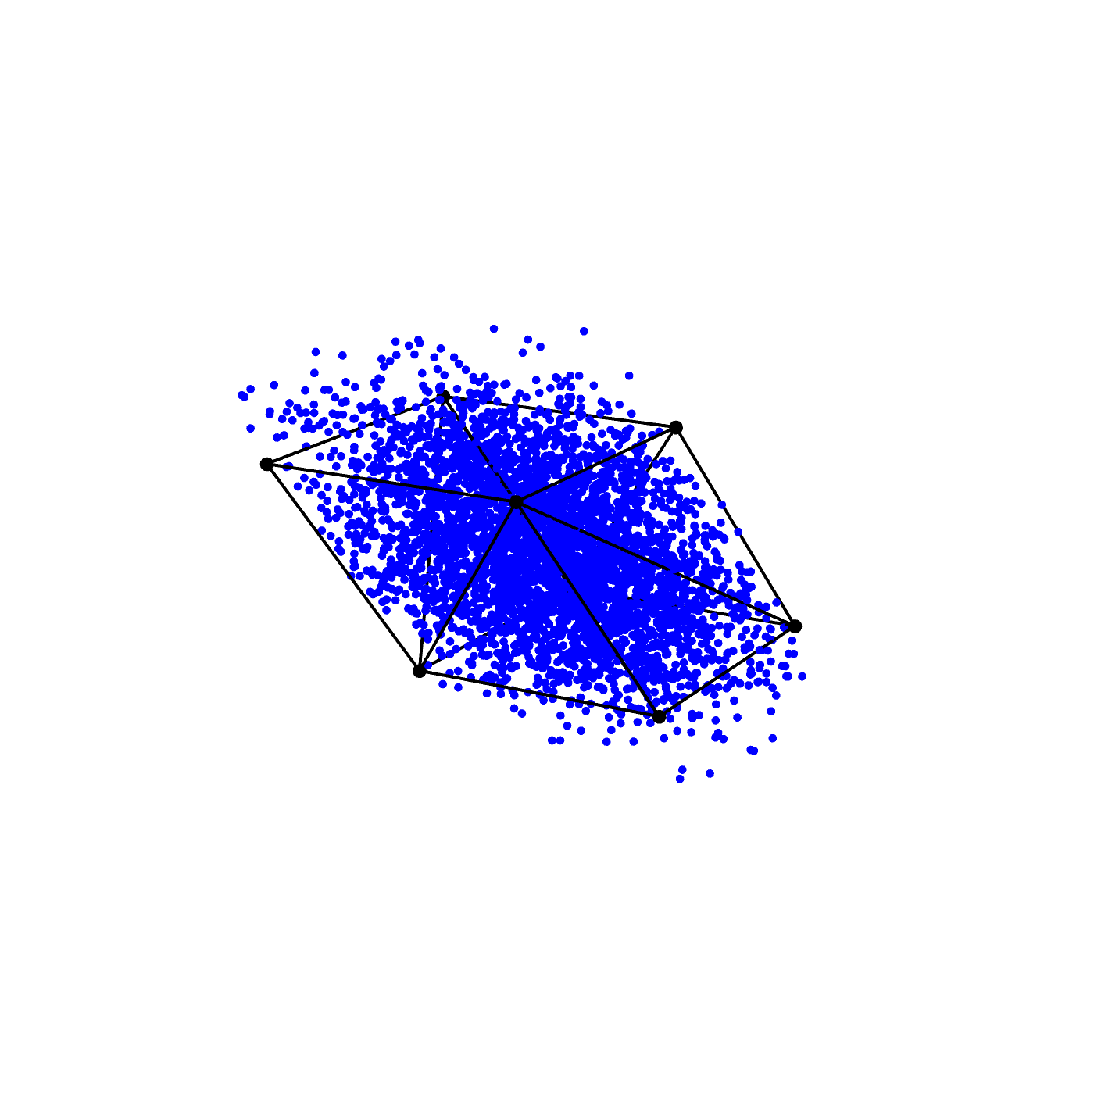
\includegraphics[width=\textwidth]{Abschlussarbeit_2021/LaTeX/images/zonotope_approximation_n3.pdf}
  \end{minipage}\hfill
  \begin{minipage}[b]{0.32\textwidth}
    \centering
    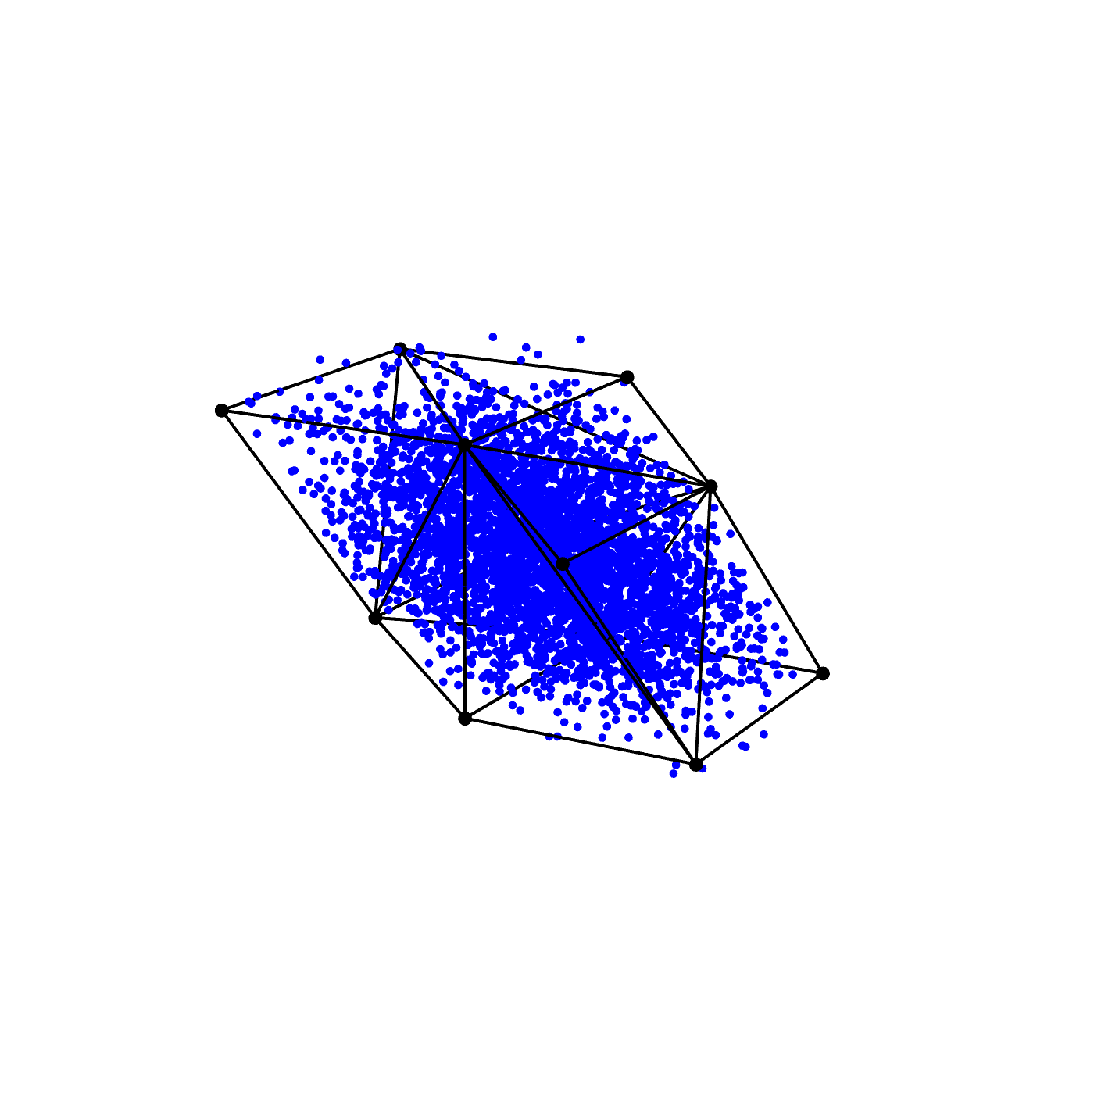
\includegraphics[width=\textwidth]{Abschlussarbeit_2021/LaTeX/images/zonotope_approximation_n4.pdf}
  \end{minipage}\hfill
  \begin{minipage}[b]{0.32\textwidth}
    \centering
    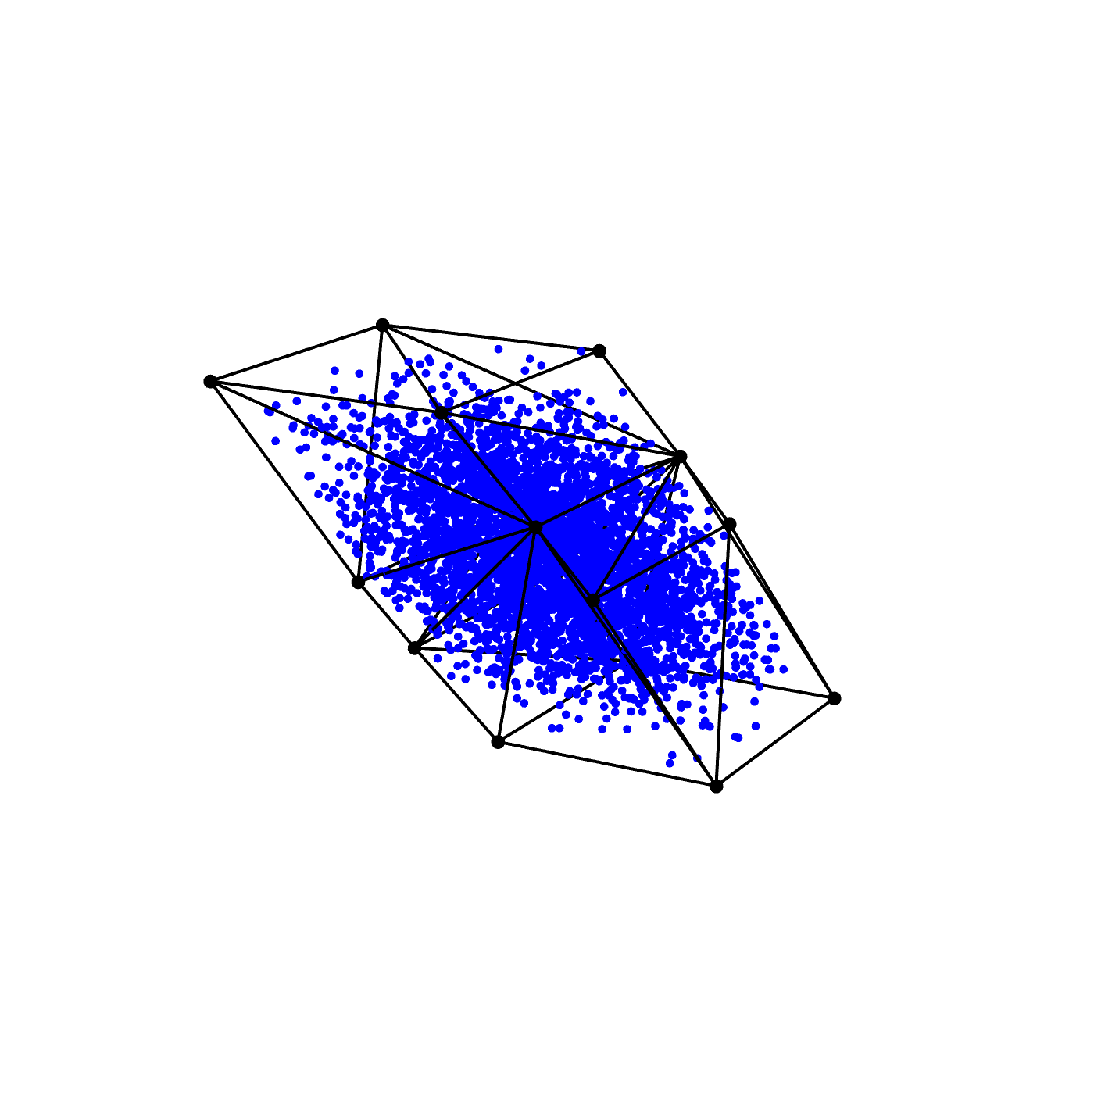
\includegraphics[width=\textwidth]{Abschlussarbeit_2021/LaTeX/images/zonotope_approximation_n5.pdf}
  \end{minipage}

  \caption{Zonotopes approximating the zonoid $\mathcal{Z}$, where $n=3$ (left), $n=4$ (center) and $n=5$ (right)}
  \label{fig:zonotopes}
\end{figure}

\todo[inline]{give approximation quality statement which should connect to the sequence $\psi_j$}

\todo[inline]{Formula for corner points?}

In the case of uniform innovations $Z_t\sim\mathcal{U}[-1,1]$ the points also lie between the hyperplanes with the same form as the central hyperplane, but with affine parts $-1$ and $1$. See Figure~\ref{fig:3d_emb_ar2}.

\begin{figure}[ht]
    \centering
    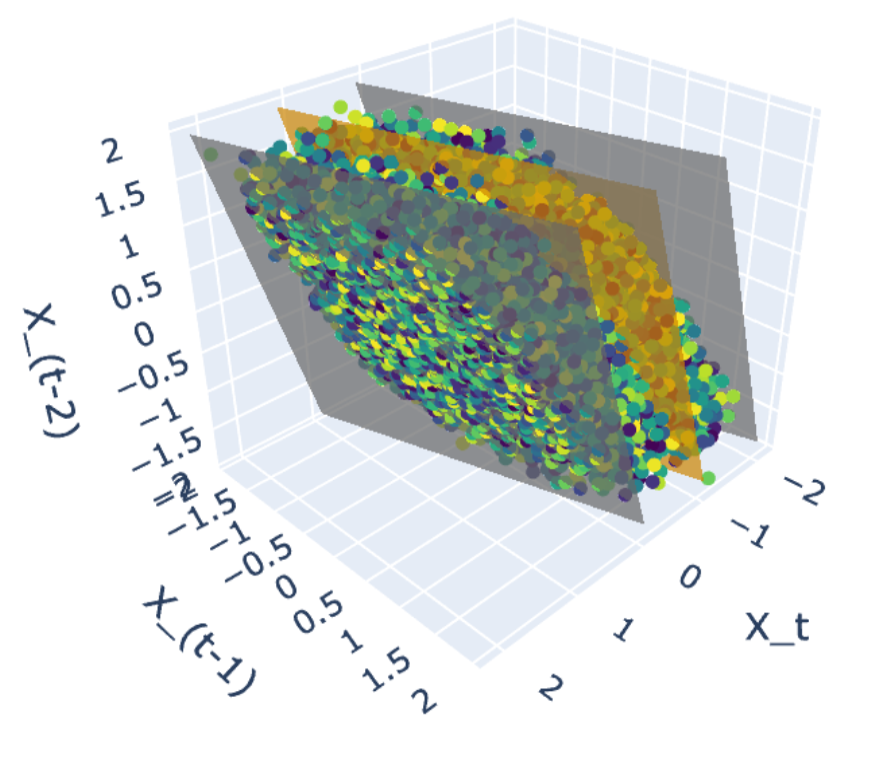
\includegraphics[width=0.5\linewidth]{Abschlussarbeit_2021/LaTeX/images/3d_emb_ar2_cropped.png}
    \caption{Sliding-window embedding ($k=3$) of an AR(2) process. The orange plane is the central plane (right side = 0), the two gray planes are the planes with affine parts -1 and 1 (due to the innovations being $\mathcal{U}[-1,1]$ distributed)}
    \label{fig:3d_emb_ar2}
\end{figure}

If $k>p+1$, the point $Y_t^{(k)}$ lies inside the intersection of multiple slabs:
\begin{align*}
    &\left\{(x_0,\dots,x_{k-1})\in\mathbb{R}^{k}:\begin{array}{l}
    -1\le x_j-\phi_1x_{j+1}-\dots-\phi_px_{j+p}\le 1,\\
    j=0,\dots,k-p-1 
    \end{array}\right\}\\&
    \bigcap_{j=0}^{k-p-1}\left\{(x_0,\dots,x_{k-1})\in\mathbb{R}^{k}:-1\le x_j-\phi_1x_{j+1}-\dots-\phi_px_{j+p}\le 1\right\}
\end{align*}

\todo[inline]{Set $p=1$ and $k=3$, visualize the intersection of slabs}

The distance between the two restricting hyperplanes is given by the formula
\begin{align*}
    d=\frac{2}{\sqrt{1+\phi_1^2+\dots+\phi_p^2}}
\end{align*}

\begin{Def}[Support function]
    Let $K\subseteq\mathbb{R}^{d}$ be a convex nonempty set. The support function of $K$ is $h_K:\mathbb{R}^d\to\mathbb{R}$, $h_K(u)=\sup\{\langle x,u\rangle:x\in K\}$.
\end{Def}

A convex body is a compact nonempty convex set. 

\begin{Lem}
    Let $K,L\subseteq\mathbb{R}^d$ be two convex bodies. Then
    \begin{align*}
        d_H(K,L)=\sup_{u\in S^{d-1}}|h_{K}(u)-h_{L}(u)|.
    \end{align*}
\end{Lem}

The support function of a zonotope is particularly easy: $h_{\mathcal{Z}_n^{(k)}}(u)=\sum_{j=0}^{n}\langle g_j^{(k)},u\rangle$. The width in direction $u$ is given by
\begin{align*}
    w_k(u)=h_{\mathcal{Z}_n^{(k)}}(u)+h_{\mathcal{Z}_n^{(k)}}(-u)=2h_{\mathcal{Z}_n^{(k)}}(u)
\end{align*}
Consider the case $k\ge p+1$. We have
\begin{align*}
    \min_{u\in S^{k-1}}w_k(u)=\frac{2}{\sqrt{1+\phi_1^2+\dots+\phi_p^2}}
\end{align*}
This minimum is attained at the finite set of points
\begin{align*}
    \left\{\pm\frac{q_r^{(k)}}{\|q_{\phi}\|_2}:r=0,\dots,k-(p+1)\right\}
\end{align*}
where $q_{\phi}=(1,-\phi_1,\dots,-\phi_p)$ and
\begin{align*}
    q_r^{(k)}=(\underbrace{0,\dots,0}_{r},1,-\phi_1,\dots,-\phi_p,0,\dots,0)\in\mathbb{R}^{k}
\end{align*}

\todo[inline]{What about $k<p+1$? Is $\min w_k(u)>2^{-1}\sqrt{1+\phi_1^2+\dots+\phi_p^2}$}

An empirical version is given by
\begin{align*}
    \hat{w}_k(u)&=\max_{t}\langle u,Y_t^{(k)}\rangle-\min_{t}\langle u,Y_t^{(k)} \rangle\\
    \hat{m}_k&=\min_{u\in S^{k-1}}\hat{w}_k(u)
\end{align*}

\todo[inline]{Give some convergence result $\hat{w}_k(u)\to w_k(u)$ or $m_k\to\hat{m}_k$}

The idea is to minimize $\hat{w}_k(u)$ over all $u\in S^{k-1}$ and examine the relation $k\mapsto \hat{m}_k$. \textcolor{red}{Unfortunately this minimization problem is very hard.}

\todo[inline]{show numerical results for $p=1,2,3,\dots$}
\todo[inline]{compare $k\mapsto\min w_k(u)$ and $k\mapsto\min\hat{w}_k(u)$}
\todo[inline]{How should the scale similarity matrix be defined?}

For such minimization problems viable methods exist, but the real problem is, that the points $Y_t^{(k)}$ do not fill the support $\mathcal{Z}_k$ well. Rigorously speaking, the convergence of the convex hull of $\mathcal{P}_k$ to $\mathcal{Z}_k$ is of the order $O((\frac{\log n}{n})^{2/(k+1)})$.

\subsection{Normally distributed innovations}

Next, we turn our attention to Gaussian innovations, which is often seen as the default case, that is, $Z_t\sim N(0,\sigma^2)$ for some $\sigma>0$. Using the MA($\infty$) representation, we see that $Y_t^{(k)}\sim\mathcal{N}(0,\Gamma_k)$ with covariance matrix
\begin{align*}
    \Gamma_k=\sigma^2\sum_{j=0}^{\infty}g_j^{(k)}(g_j^{(k)})^{T}
\end{align*}
The covariance matrix plays an important role in describing the geometry of the point cloud $\mathcal{P}_k$. Let $E_c=\{y\in\mathbb{R}^k:y^{T}\Gamma_k^{-1}y\le c\}$ be the ellipsoid of size $c>0$. Then for all $\alpha\in(0,1)$ we have
\begin{align*}
    E_{c_{\alpha}}\in\arg\min\left\{\operatorname{Vol}(A):\mathbb{P}(Y\in A)\ge\alpha:A\subseteq\mathbb{R}^{k}\right\}
\end{align*}
That is, the ellipsoid with size $c_{\alpha}$ is the set with minimum volume, such that the probability that $Y$ is inside $E_{c_{\alpha}}$ is at least $\alpha$.

\todo[inline]{find reference or prove}

\subsection{Heavy-tailed innovations}

\todo[inline]{TBD}

\subsection{Intrinsic Volumes}

\todo[inline]{Handbook of Convex Geometry}

We have a zonotope $Z^{(n)}_k=\sum_{j=0}^{n}g_j[-1,1]$ with \textcolor{red}{unknown} vectors $g_j\in\mathbb{R}^k$. Here, $k$ is the embedding dimension. The $j$-th quermassintegral of $Z^{(n)}_k$, denoted by $W_j(Z^{(n)})$ are defined as coefficients that fulfill
\begin{align*}
    \operatorname{Vol}(Z^{(n)}_k+tB)=\sum_{j=0}^{k}\binom{k}{j}W_j(Z^{(n)}_k)t^{j}
\end{align*}
where $B=B(0,1)=\{x\in\mathbb{R}^k:\|x\|\le1\}$. The $j$-th intrinsic volume is defined by
\begin{align*}
    V_j(Z^{(n)}_k)=\binom{k}{j}\frac{W_{k-j}(Z^{(n)}_k)}{\kappa_{k-j}}, && j=1,\dots,k
\end{align*}
It can be shown that the $j$-th intrinsic volume can by computed by the formula
\begin{align*}
    V_j(Z^{(n)}_k)=2^{j}\sum\limits_{I\subseteq\{0,\dots,n\},|I|=j}\sqrt{\det{(G_I^TG_I)}}
\end{align*}

\subsection{Scale selection for Geometric Approach}

We can fill our scale similarity matrix $\Sigma^{(n)}=\left(\Sigma^{(n)}_{kl}\right)$ with the entries
\begin{align*}
    \Sigma^{(n)}_{kl}=f\left(Z_k^{(n)}\right)+f\left(Z_l^{(k)}\right)-f\left(Z_k^{(n)}\oplus Z_l^{(n)}\right),
\end{align*}
where $\oplus$ is an operation that takes two zonotopes and combines them into a new zonotope. Such an operation can be the following:
\begin{align*}
    Z_k^{(n)}\oplus Z_{l}^{(n)}=\sum_{j=0}^{n}[-1,1]\phi_{k}\left(g_j^{(k)}\right)+
    \sum_{j=0}^{n}[-1,1]\phi_l\left(g_j^{(l)}\right)
\end{align*}
Here, the sum is understood as Minkowski-sum. The Minkowski-sum of two zonotopes is again a zonotope, that is, $Z_k^{(n)}\oplus Z_l^{(n)}$ is again a zonotope. Prior to that we have to apply an embedding $\phi_k:\mathbb{R}^{k}\to\mathbb{R}^{k_{\max}}$, $k=1,\dots,k_{\max}$ with $\phi_k((x_1,\dots,x_k))=(x_1,\dots,x_k,x_{k+1},\dots,x_{k_{\max}})$ (the first $k$ coordinates are preserved).


We can choose $f=V_j$, $j=1,\dots,k$ as functional.

\todo[inline]{Big Question: How to generalize this approach for a wide class of innovation distributions? We only get the nice zonotope formulas because of uniform innovations}

\todo[inline]{Maybe find a class of distributions where the highest density region (or minimum volume set) has a nice geometric shape and compute the intrinsic volumes of that shape}





\section{Numerical Results}

\begin{itemize}
    \item AR($p$) for $p=1,2,3$
    \item different innovations
    \item compare with classical order selection
    \item finite sample stability $(X_1,\dots,X_T)$, $T=200,500,1000$
\end{itemize}





